\documentclass[11pt]{article}
%ACENTOS
\usepackage[utf8]{inputenc}
\def\figurename{Fig.}
\def\tablename{Tabla}
\def\refname{Referencias}
\setlength{\parskip}{1em}

%PAQUETES
\usepackage{amsfonts,amsmath,amssymb}    % need for subequations
\usepackage{amsmath,latexsym}
\usepackage{graphics,color}
\usepackage{graphicx}
\usepackage{algpseudocode}
\usepackage[most]{tcolorbox}
\usepackage{hyperref} %Para colocar direcciones Web
\usepackage{booktabs} % Tablas
\usepackage[thinc]{esdiff} % Derivadas

%MARGEN
\setlength\topmargin{-0.5in}
\addtolength\oddsidemargin{-0.5in}
\setlength{\textheight}{23cm}
\setlength{\textwidth}{16cm}

%VARIABLES
\newcommand{\N}{\mathbb N}
\newcommand{\Z}{\mathbb Z}
\newcommand{\R}{\mathbb R}
\newcommand{\C}{\mathbb C}
\providecommand{\norm}[1]{\lVert#1\rVert}
%COLORES
\newcommand{\rojo}[1]{\textcolor[rgb]{1.00,0.00,0.00}{#1}}
\newcommand{\azul}[1]{\textcolor[rgb]{0.00,0.00,1.00}{#1}}
 
  
\begin{document}

\begin{center}
 \Large \underline {\\ \\Tarea 1: Ceros de funciones} \\ \medskip
 \small  {Elaborado por Giselt Parra}\\ 
 \footnotesize{16 de Octubre de 2020}
\end{center}


\begin{center} \Large {1. Métodos} \end{center}

\justify
%Métodos para hallar raíces de funciones $f: R \to R:$

% BISECCION
{\large (a) Método de la Bisección}

Sea una función f continua en un intervalo cerrado [a,b] donde se encuentra una raíz, el método de la bisección consiste en:

\begin{enumerate}
	\item[\textperiodcentered] Calcular el punto medio (c) del intervalo. Si $f(c)\neq 0$, se generan dos subintervalos.
	\item[\textperiodcentered] Seleccionar el subintervalo que contenga la raiz. Para esto se comparan los signos de las alturas del extremo del subintervalo, si son distintos entonces existe un punto de corte con el eje x dentro de él.
	\item[\textperiodcentered] Se repite el procedimiento tomando el subintervalo seleccionado como el intervalo a evaluar.
\end{enumerate}
Este proceso se repite hasta que la longitud del intervalo sea igual o menor a la precisión 

\begin{center}
    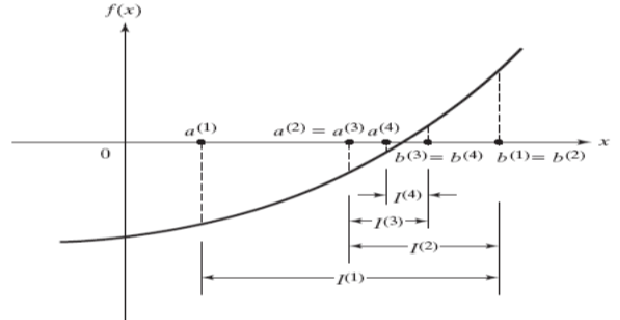
\includegraphics[keepaspectratio, width=8cm]{BM.png}
    \caption{\\}
\end{center} 

\vspace{0.5cm}


% REGULA FALSI                   CHEEEEEEEEEEEEEEEEEQUE
{\large (b) Método de Regula Falsi}

El método de la Regula Falsi o también conocido como el método de Falsa Posición trabaja de una manera similar al método de la bisección donde en un intervalo [a,b] se traza una recta secante que va desde (a, f(a)) a (b, f(b)). Siendo $f(a)f(b)<0$ se garantiza la existencia de una raíz en ese intervalo. Esta recta secante cortará en algún punto con el eje x y dicho punto (c) si no cumple que $f(c) = 0$ o $|f(c)|<\xi$ entonces se deben comparar las alturas, si $f(c)f(a)>0$ entonces c será el extremo inferior del intervalo en la siguiente iteración. En el caso contrario, será el extremo superior.

Para calcular este punto c, cada iteración parte de trazar la recta secante entre (a, f(a)) y (b, f(b)). Sabemos que la recta secante entre (a, f(a)) y (b ,f(b)) es igual a la secante entre  cualquiera de estos dos puntos del intervalo con el punto c que queremos calcular:
    $$\frac{f(a)-f(b)}{a-b} = \frac{0-f(b)}{c-b} = \frac{0-f(a)}{c-a} $$
	%$$(f(a)-f(b))(c-b) = (0-f(b))(a-b) $$ 
 Despejamos c:
	$$c = b - f(b) \frac{a-b}{f(a)-f(b)} = a - f(a) \frac{a-b}{f(a)-f(b)}$$
	
\begin{center}
    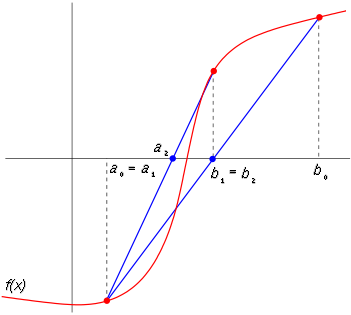
\includegraphics[keepaspectratio, width=7cm]{RFM.png}
    \caption{\\}
\end{center} 

\vspace{0.5cm}


% SECANTE
{\large (c) Método de la Secante}
%Conforme estos puntos se acercan y su distancia se reduce a cero, la recta adquiere el nombre de recta tangente.

A diferencia del método de Newton, este método se hace a través rectas secantes a la función cuyo punto de corte con el eje x se acercará a la raíz. La ventaja de este método es que sólo se necesita evaluar la función por cada iteración a diferencia del método de Newton que por cada iteración evalúa la función y su derivada.

\begin{center}
    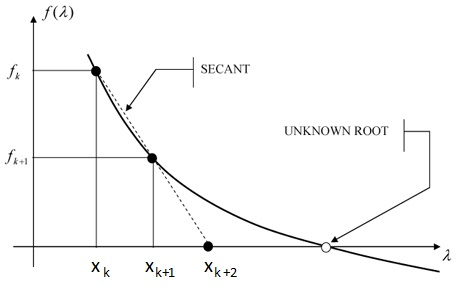
\includegraphics[keepaspectratio, width=8cm]{SM.jpg}
    \caption{\\}
\end{center} 

\begin{enumerate}
	\item[\textperiodcentered] Se toman dos puntos iniciales y como ha sido mencionado previamente, en vez de usar la derivada de la función, tomaremos la recta secante a la función que se genera con estos dos puntos
 $$x_{k+1} = x_k - \frac{f(x_k)}{ \frac{f(x_{k-1})-f(x_k)}{x_{k-1}-x_k} }\hspace{0.5cm} \forall k \in N$$ 
\end{enumerate}
Se iterará hasta obtener un punto cuya altura sea menor al rango de error aceptable o hasta que k alcance el número máximo de iteraciones previamente definido.
\vspace{0.5cm}


% NEWTON
{\large (d) Método de Newton}
%sólo posee convergencia local.

Este método iterativo se realiza por medio del trazo de rectas tangentes a la función hasta que el punto de corte con el eje x de estas rectas sea o se acerque lo suficiente a la raíz de la función. Los pasos para conseguir el cero de la funcion son los siguientes:

\begin{center}
    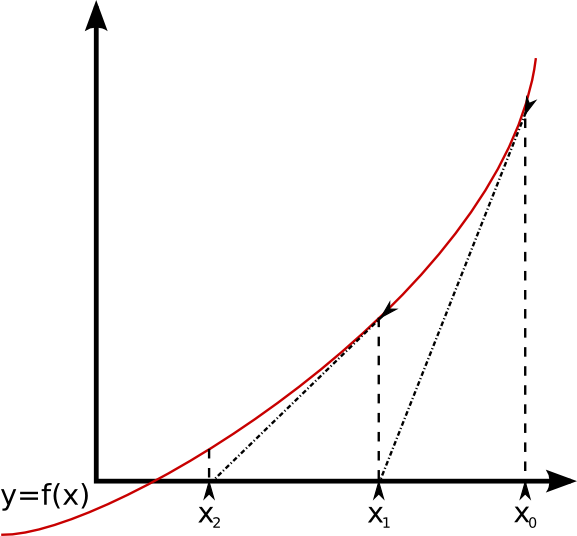
\includegraphics[keepaspectratio, width=7cm]{NM.png}
    \caption{\\}
\end{center} 

\begin{enumerate}
	\item[\textperiodcentered] Se toma un punto inicial $x_0 \in [a,b] / f'(x_0)\neq 0$ y se traza la recta tangente a la función
	$$y - f(x_o) = f'(x_o)(x-x_o)$$
	\item[\textperiodcentered] Para calcular el siguiente punto, reemplazamos y=0 en la expresión anterior y nos queda: $$x = x_1 = x_0 - \frac{f(x_0)}{f'(x_0)}$$
	\item[\textperiodcentered] Podemos generalizar para el resto de las iteraciones: $$ x_{k+1} = x_k - \frac{f(x_k)}{f'(x_k)}\hspace{0.5cm} \forall k \in N$$ 
	
	Se iterará hasta obtener un punto cuya altura sea menor al rango de error aceptable o hasta que k alcance el número máximo de iteraciones previamente definido.
\end{enumerate}
\vspace{0.5cm}


% PUNTO FIJO
{\large (e) Método del Punto Fijo}

En este método se tiene una función f donde $f(x) = 0$ y las iteraciones consisten aproximarse a la raíz igualandola a una función g de modo que $x = g(x)$. Se considerará punto fijo al punto que cumpla que $f(x) = x - g(x)$. La manera en la que se procede es la siguiente:

\begin{enumerate}
	\item[\textperiodcentered] Se escribe f como f(x) = 0.
	\item[\textperiodcentered] Expresar f en función de $x = ...$ de tal modo que dicha x que está del lado izquierdo de la igualdad sea $x_{k+1}$ y dependa del iterador anterior $x_k$.
\end{enumerate}
Para la primera iteración se iniciará con un $x_0$ dado y se iterará hasta converga.

El método de Newton es un caso especial de este método donde $g(x) = x - \frac{f(x)}{f’(x)}$.
\vspace{0.75cm}

\begin{center} \Large {2. Convergencia} \end{center}

% BISECCION
{\large (a) Método de la Bisección}

Este método tiene la ventaja de existir una raiz en el intervalo dado, es segura la convergencia aunque esta sea lenta. De esto podemos asegurar que la sucesión de intervalos generados coverge a cero y se reduce a la mitad por cada par de iteraciones sucesivas. Dado a que es secuencialmente constante la velocidad en que la sucesion de intervalos converge, su velocidad es q-lineal con r = 1 y C = 0.5. 
$$\lim_{k \to \infty}{\frac{|x_{k+1}-x_*|}{|x_k-x_*|}} = \frac{1}{2}$$

Sabemos que la diferencia entre la raíz de la función y el $x_k$ es menor a la logitud del intervalo de incertidumbre en la iteración k y como este intervalo converge de forma q-lineal entonces por defición la velocidad en la que el método converge a cero será r-lineal, esto quiere decir que la secuencia de los ${x_k}$ para ${k\geq 0}$ posee una convergencia no monótona.
\vspace{0.5cm}

% BISECCION
{\large (b) Método de la Regula Falsi}

Sea f continua en el intervalo dado [a, b] con una raíz, si existe su segunda derivada y f es convexa entonces uno de los puntos a o b permanecerá fijo en todas las iteraciones mientras el otro varía y se acerque lo suficiente a la raíz.

El error se calcula de la siguiente forma tomando a como el punto que permanece fijo:
$$|x_{k+1}-x_*| = C |x_{k}-x_*| |x_{k-1}-x_*|$$ 
$$|x_{k+1}-x_*| = C |x_{k}-x_*| |a-x_*|$$ 

donde $C = \frac{f''(x_*)}{2f'(x_*)}$ y con $M = C|a-x_*|$ siendo una constante nos queda:
$$\lim_{k \to \infty}{\frac{|x_{k+1}-x_*|}{|x_k-x_*|}} = M$$
por lo que con r = 1 y $0 \leq M \leq 1 $ la velocidad es q-lineal

\vspace{0.5cm}

% BISECCION
{\large (c) Método de la Secante}
%Sea f'' continua y x_∗ un cero simple de f. Hay una vecindad de x_∗ y una constante C tales que si el método de la Secante se inicia en esa vecindad, los iterados generados por dicho método convergen a x_∗ y satisfacen


El metódo de la Secante comparte la formula de iteración con Regula Falsi 
$$\lim_{k \to \infty}{\frac{|x_{k+1}-x_*|}{|x_k-x_*|}} = M$$

con la diferencia de que se usan dos iteradores para calcular el nuevo punto por lo que nos queda:

$$\lim_{k \to \infty}{\frac{|x_{k+1}-x_*|}{|x_k-x_*| |x_{k-1}-x_*|}} = M$$

para propósitos de simplificar visualmente los siguientes calculos escribiremos $|x_{k+1}-x_*| = \xi_{k+1}$, $|x_{k}-x_*| =|\xi_{k}|$ y $|x_{k-1}-x_*| = |\xi_{k-1}|$ y reescribiremos la expresión con la intención de encontrar el valor de r. Partimos de lo siguiente

$$\frac{|\xi_{k+1}|}{|\xi_{k}|^r} = t_k \to |\xi_{k+1}| = |\xi_{k}|^r t_k = t_k(s_{k-1}|\xi_{x-1}|^r)^r = t_k t^r_{k-1}|\xi_{x-1}|^{r^2} $$

regresando a nuestra fórmula original
$$\frac{|\xi_{k+1}|}{|\xi_{k}||\xi_{k-1}|} = 
\frac{t_k t^r_{k-1} |\xi{k-1}|^{r^2}}{t_{k-1} |\xi_{x-1}|^r |\xi_{x-1}|} = t_k t^{r-1}_{k-1} |e_{k-1}|^{r^2 - r -1}$$

de manera analoga sabemos que $t^{r-1}_{k-1} = \frac{|\xi_{k}|}{|\xi_{k-1}|^r}$ y que $\xi \to 0$ para cualquier valor de $r > 0$ por lo que nos queda $t_k |e_{k-1}|^{r^2 - r -1}$ y para encontrar el valor de r sólo debemos hallar la raíz de $r^2 - r -1$. Dado a que r debe ser un número positivo, tomaremos la solución positiva $r = \frac{1+\sqrt{5}}{2}$.

\vspace{0.5cm}

% BISECCION
{\large (d) Ḿetodo de Newton}

Para estudiar la convergencia en el método de Newton debemos tomar en cuenta la multiplicidad (m) de la raíz de la función que denominaremos $x_*$. En el caso de que la función tenga una raíz simple tenemos lo siguiente:

\\\textbf{Teorema}: Sea $f:[a,b]\to R$ con segunda derivada y continua en el intervalo [a,b], si se cumple que:

\begin{enumerate}
\item[\textendash]$f(a)f(b) < 0$
\item[\textendash]$f'(x_*) \neq 0 \hspace{0.5cm} \forall x \in [a,b]$ 
\item[\textendash]$f''(x_*) \neq 0 \hspace{0.5cm} \forall x \in [a,b]$
\end{enumerate}
De escogerse un punto inicial $x_0$ tal que $f(x_0)f''(x_0)>0$, se garantiza que las sucesivas aproximaciones del método convergen a la raíz con r = 2, por tanto la velocidad de convergencia será q-cuadrática, esto significa que se duplica el número de dígitos de precisión con cada iteración.
\\El error se calculará de esta manera:
$$ |x_{x+1}-x_*| \leq C |x_k-x_*|^2  \hspace{0.5cm} 
C = \frac{f''(x_*)}{2f'(x_*)}$$
%$$\equiv \lim_{k \to \infty} \frac{|x_{x+1}-x_*|}{|x_k-x_*|^2} \leq C$$

Para el caso donde $f^i(x_*) = 0$ con $2\leq i \leq m$, el método posee convergencia q-orden m.

Cuando $f(x_*)= f'(x_*) = ... = f^{m-1}(x_*)= 0$ entonces $x_0$ tiene multiplicidad $m$ y la velocidad del método convergencia es lineal por lo que es más lento que el caso donde la función tiene raíz simple. Sin embargo, existe una manera de incrementar la velocidad del método y consiste en multiplicar la multiplicidad al intervalo que existe entre el $x_k$ y $x_{k+1}$ en cada iteración k
$$x_{k+1} = x_k - \frac{mf(x_k)}{f'(x_k)}$$
\vspace{0.5cm}

%           CHEEEEEEEEEEEEEEEEEEEQUEAR ABAJO






{\large (e) Método del Punto Fijo}

No todas las funciones g que se derivan despejar una x en f tienen la misma velocidad de convergencia, de hecho, es de importancia destacar que es posible que algunas de estas funciones no lleguen a la solución y por tanto, la sucesion de ${x_k}_{\forall k \in N}$ no es convergente. La manera de determinar si g convergerá y de hacerlo, a qué velocidad lo hará es con la derivada de la función g. Si en algún punto existe un $x_*$ perteneciente al dominio de f tal que $|g'(x_*)|<1 $ entonces g convergerá.

Una particularidad de este método es que saber que la derivada de g tendrá ciertos valores en la raíz de la función da información sobre la velocidad de convergencia. 
\begin{enumerate}
\item[\textendash] Si $g'(x) = 0 $, entonces la velocidad es q-cuadrática. 
\item[\textendash] Si $g''(x) = 0 $, entonces la velocidad es q-orden 3. 
\item[\textendash] Si $g'''(x) = 0 $, entonces la velocidad es q-orden 4. 

y así sucesivamente.
\end{enumerate}
\vspace{1cm}

\begin{center} \Large {3. Métodos programados | Criterios de parada}\end{center}

\begin{tcolorbox}[colframe=blue!35!black, title=Código]
    metodos.m
\end{tcolorbox}

\begin{enumerate}
\item[\textendash] Para los métodos que trabajan en función de reducir intervalos como lo son el de la Bisección y Regula Falsi, dado a que se garantiza que existe una raíz dentro del intervalo, si el método no se detiene cuando $f(c) <= \xi$ entonces deberá hacerlo cuando $|a-b| <= \xi$ que quiere decir que el intervalo que acota la raíz es lo suficientemente pequeño.
\item[\textendash] Para los métodos donde se trazan rectas tangentes o secantes, la estrategia de parar cuando $|a-b| <= \xi$ no garantiza que se ha logrado la aproximación deseada por lo que se tomará en cuenta las alturas en los puntos a evaluar garantizando que $x_k$ se tomará como cero de función cuando $f(x_k) <= \xi$.
\item[\textendash] Para el método de Punto Fijo se iterará hasta conseguirse un punto c tal que $g(c) - c = f(c)$.

\end{enumerate}


\vspace{1cm}
\begin{center} \Large {4. Ejemplos} \end{center}
{\large Ejemplos en métodos cerrados}
\begin{center}
    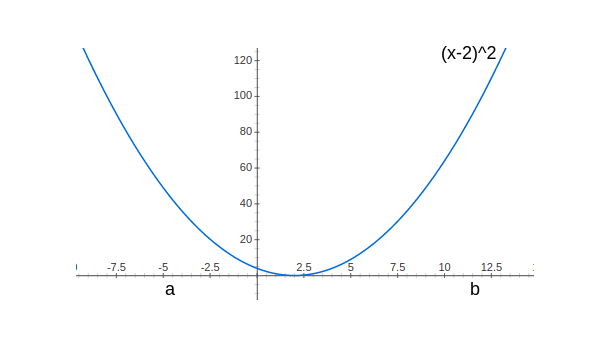
\includegraphics[keepaspectratio, width=7cm]{Problema_MetodoAbierto1.png}
    \caption{\\}
\end{center}   
Los métodos de Bisección y Regula Falsi no pueden hallar raices que a su vez sean minimo o máximo de la función dado a que en bisección ningún intervalo se detectará como contenedor de la raiz y cualquier recta secante que se trace en f no cortará con el eje x. Por esta razón la condición para garantizar la convergencia global en estos métodos es que la altura de los extremos de los intervalos tengan signos opuestos.


\begin{center}
    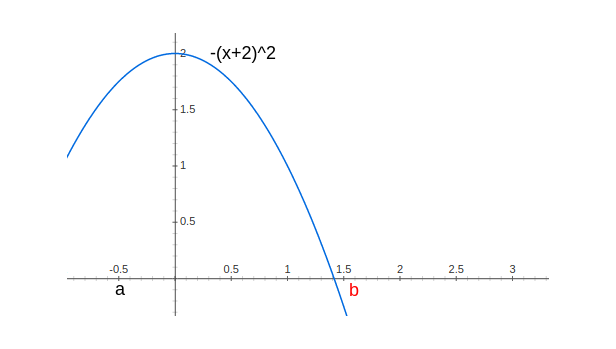
\includegraphics[keepaspectratio, width=8cm]{Problema_MetodoAbierto2.png}
    \caption{\\}
\end{center}   
El peor de los casos en los métodos que consisten reducir intervalos es cuando el valor a buscar se encuentra muy cerca de uno de los extremos del intervalo. Esto significa que requerirá una mayor cantidad de iteraciones para aproximarse a diferencia de que dicho valor estuviera ubicado cerca de los valores centrales del intervalo.

\begin{center}
    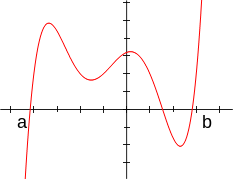
\includegraphics[keepaspectratio, width=8cm]{Problema_MetodoAbierto3.png}
    \caption{\\}
\end{center}  
$f(a)f(b)<0$ no garantiza que exista un cero de función único en el intervalo [a,b] sino la existencia de un número impar de cortes con el eje x.

{\large Ejemplos en métodos abiertos}
\begin{center}
    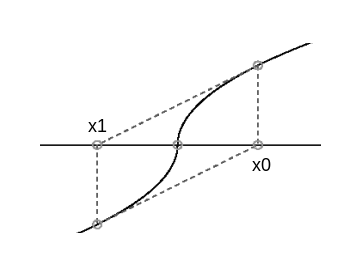
\includegraphics[keepaspectratio, width=7cm]{Problema_MetodoCerrados.png}
    \caption{\\}
     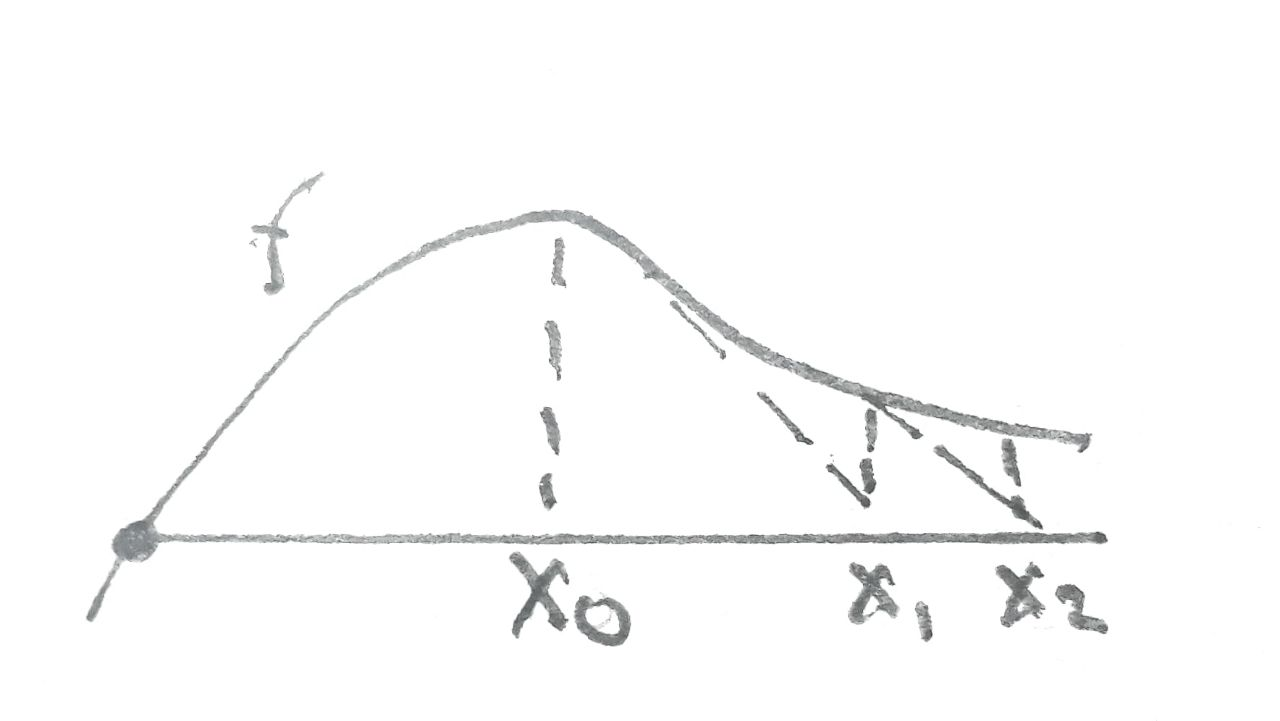
\includegraphics[keepaspectratio, width=7cm]{Problema_MetodoCerrados2.jpg}
    \caption{\\}
     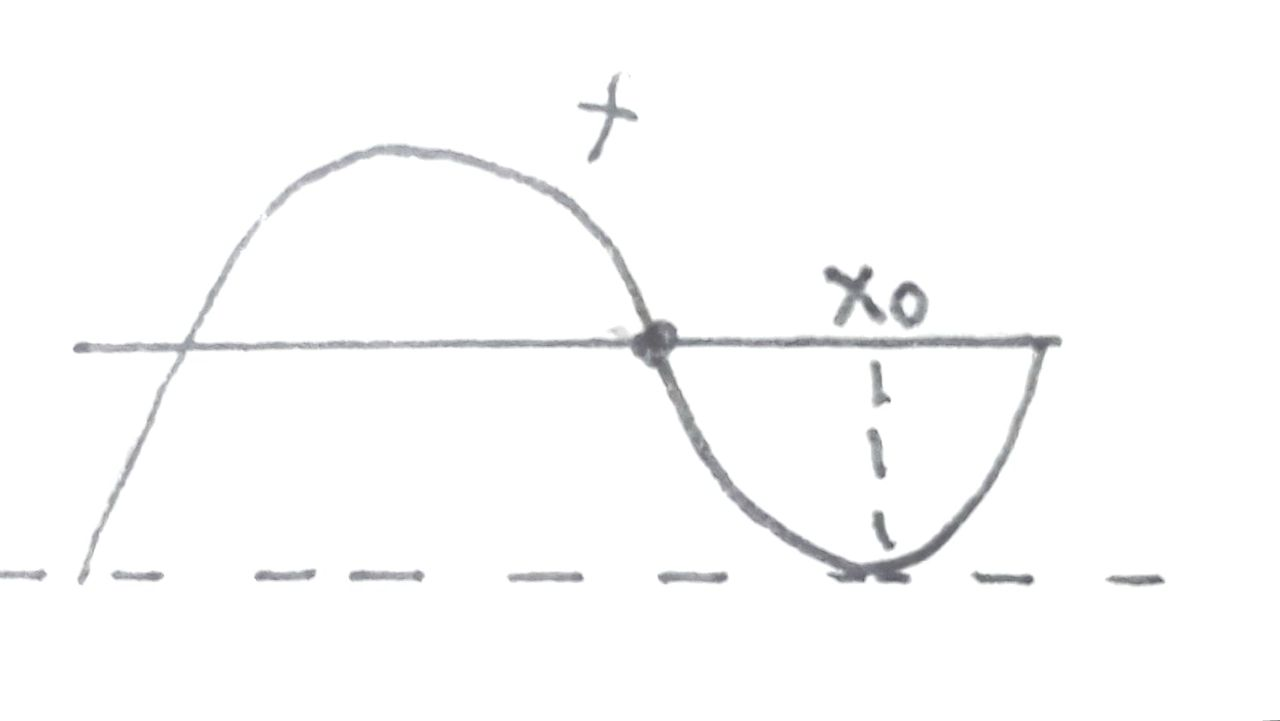
\includegraphics[keepaspectratio, width=7cm]{Problema_MetodoCerrados3.jpg}
    \caption{\\}
\end{center}   
Se puede dar este inconveniente en el método de Newton donde la asignación de nuevos puntos sea cíclica, los iteradores se alejen de la raíz o la tangente nunca corte con el eje x. Para esto, aparte de asegurase de tomar un iterador incial lo suficientemente cerca, se puede tomar la función y comprobar que $f'(x) \neq 0$ en su dominio. 

\begin{center}
    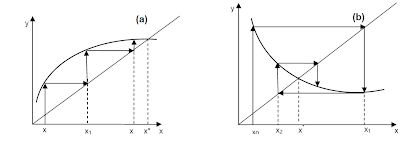
\includegraphics[keepaspectratio, width=9cm]{Di.png}
    \caption{\\}
\end{center}  
En el caso del método de Punto Fijo, la convergencia está totalmente relacionada con el comportamiento de la función f y de la función g. Gráficamente lo que se ve en la figura es lo que ocurre cuando f junto a g cumplen las condiciones para alcanzar una convergencia local y la forma más simple de comprobar esto es por medio de la derivada de g.
\vspace{1cm}
\begin{center} \Large {5. Velocidad de convergencia ilustrada} \end{center}
\begin{tcolorbox}[colframe=blue!35!black, title=Código]
    graficaError.m
\end{tcolorbox}
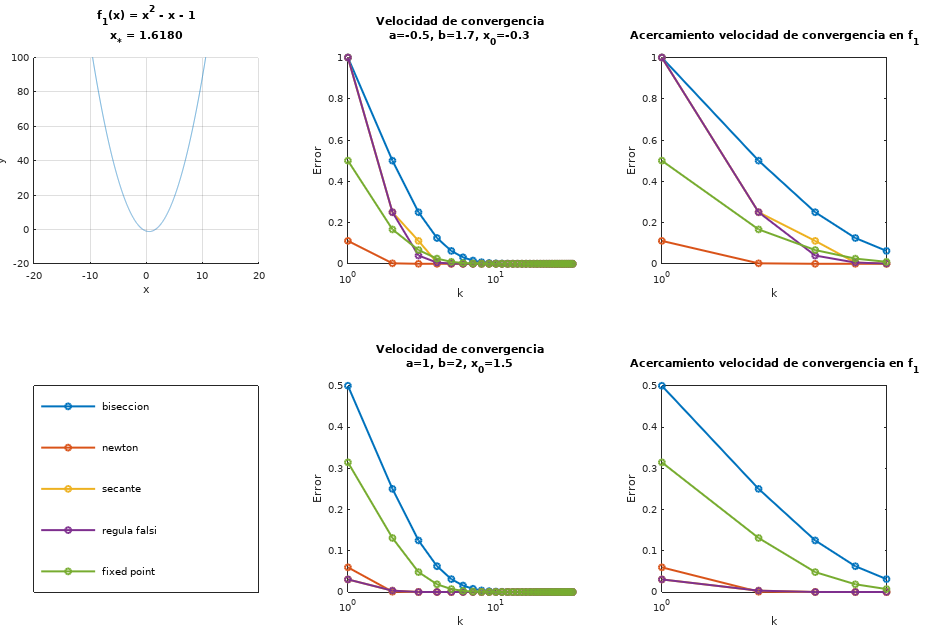
\includegraphics[keepaspectratio, width=15cm]{Error1.png}
\caption{\\}
Para la función $f_1$ se hicieron dos pruebas con el fin de evidenciar la mejora en el resultados de estos métodos dependiendo de la data de entrada. En el primer caso se tomó un intervalo grande con el valor a hallar muy cerca de uno de los extremos del intervalo y con un iterador inicial en un punto lejano a la raíz. Por el otro lado, se ejecutaron los métodos dentro de un entorno más cercano a la raíz y procurando dejar a la misma en un punto cercano al valor medio de estos valores. Los métodos Secante, Regula Falsi y Punto Fijo redujeron el número de iteraciones necesarias a la mitad, mientras que los métodos Biseccion y Newton lograron converger una iteración menos respecto a la primera prueba hecha.
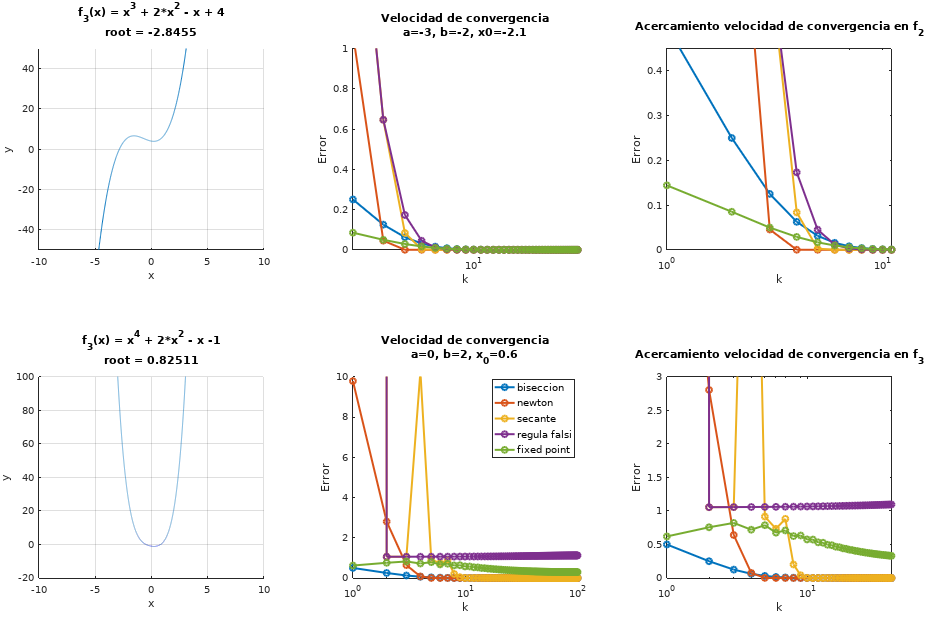
\includegraphics[keepaspectratio, width=15cm]{Error2.png}
\caption{\\}
Como en el caso general se utilizó la función $f_3$ donde se detalla (y como en el resto de los gráficos) que el método de Newton junto al método de Secante son los primeros en converger, luego en unas iteraciones más Regula Falsi y Punto Fijo convergen y por último el método de la Bisección. 

Como se puede visualizar, para $f_4$ los métodos de Punto Fijo y Regula Falsi exceden el máximo número de iteraciones preestablecido sin llegar a la convergencia. Esto se debe a que la funcion utilizada para la ejecución $g(x) =(-2x^2 + x + 1 )^\frac{1}{4} $ no cumple que $|g'(x_*)| < 1$ por lo tanto los iterados no convergen a $x_*$. Mientras, para el método Regula Falsi docurre que entre el punto a hallar y los iteradores iniciales existe un punto c cuya derivada es igual a cero, por tanto la recta secante en ese punto no cortará el eje x y por lo tanto el método falla.


\vspace{1cm}


\begin{center} \Large {6. Cuadro comparativo} \end{center}
\begin{center}
    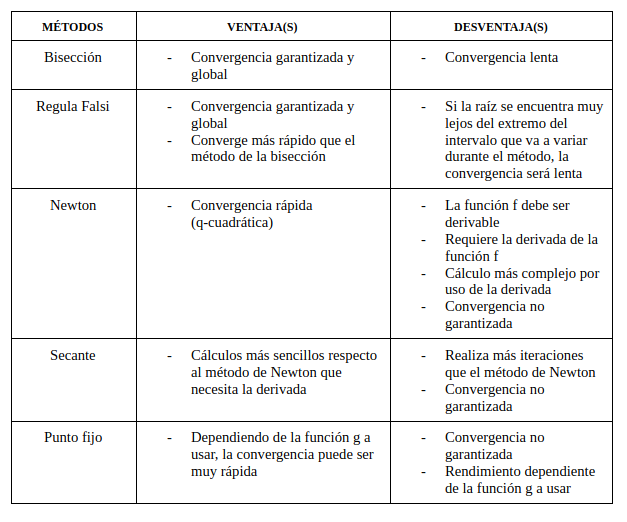
\includegraphics[keepaspectratio, width=15cm]{Cuadro.png}
    \caption{\\}
\end{center}   

Escogencia de métodos:
\begin{enumerate}
\item[\textendash] En el caso de que se requiera efectividad por encima de velocidad de convergencia, la escogencia sería por los métodos de la bisección y regula falsi ya que si las condiciones están dadas, el método gerantiza convergencia global.
\item[\textendash] Si dentro del intervalo se garantiza que no existe ningún punto cuya derivada sea igual a cero, los métodos de Newton y Secante serían los más adecuados.
\item[\textendash] A nivel de costo computacional, si el número de iteraciones entre el método de Newton y el método de la Secante no es muy grande, el método de la Secante resulta más adecuado. Lo mismo ocurre si no se tiene la derivada de la función a evaluar.
\end{enumerate}

\end{document}
